\documentclass{article}
\usepackage{blindtext}

\usepackage[top=1in, bottom=1in, left=1in, right=1in]{geometry}

\usepackage{amsmath}
\usepackage{graphicx}
\usepackage{commath}
\usepackage{siunitx}


\usepackage[b]{esvect}

\newcommand{\de}{\mathrm{d}}

\begin{document}
\title{Homework 5}
\author{Xueqi Li}
% \date{Feb 4, 2017}
% \email{xueqi.li@stonybrook.edu}

% \begin{abstract}
% Consider a vector (given with respect to a fixed Cartesian basis). Here $t$ means time.
% \[
% \vv{r}(t) = \sin(\pi t)\hat{x} + \cos(\pi t)\hat{y} - \sqrt{7}\hat{z}
% \]
% \end{abstract}

\maketitle

\begin{enumerate}
    \item Consider a mass $m$ hangs in the air suspended by four identical springs under a table. The other end of the spring are attached to the corners of the table; the table is square and its sides have length $d$.
    \begin{enumerate}
        \item sketch this arrangement.
        \item If the spring have spring constant $k$ and the spring are idea, i.e., the unstretched length is zero: $l = 0$, what is the potential energy?
        \item What is the equilibrium point?
        \item What are effective spring constants $k_x, k_y, k_z$

        \begin{center}
            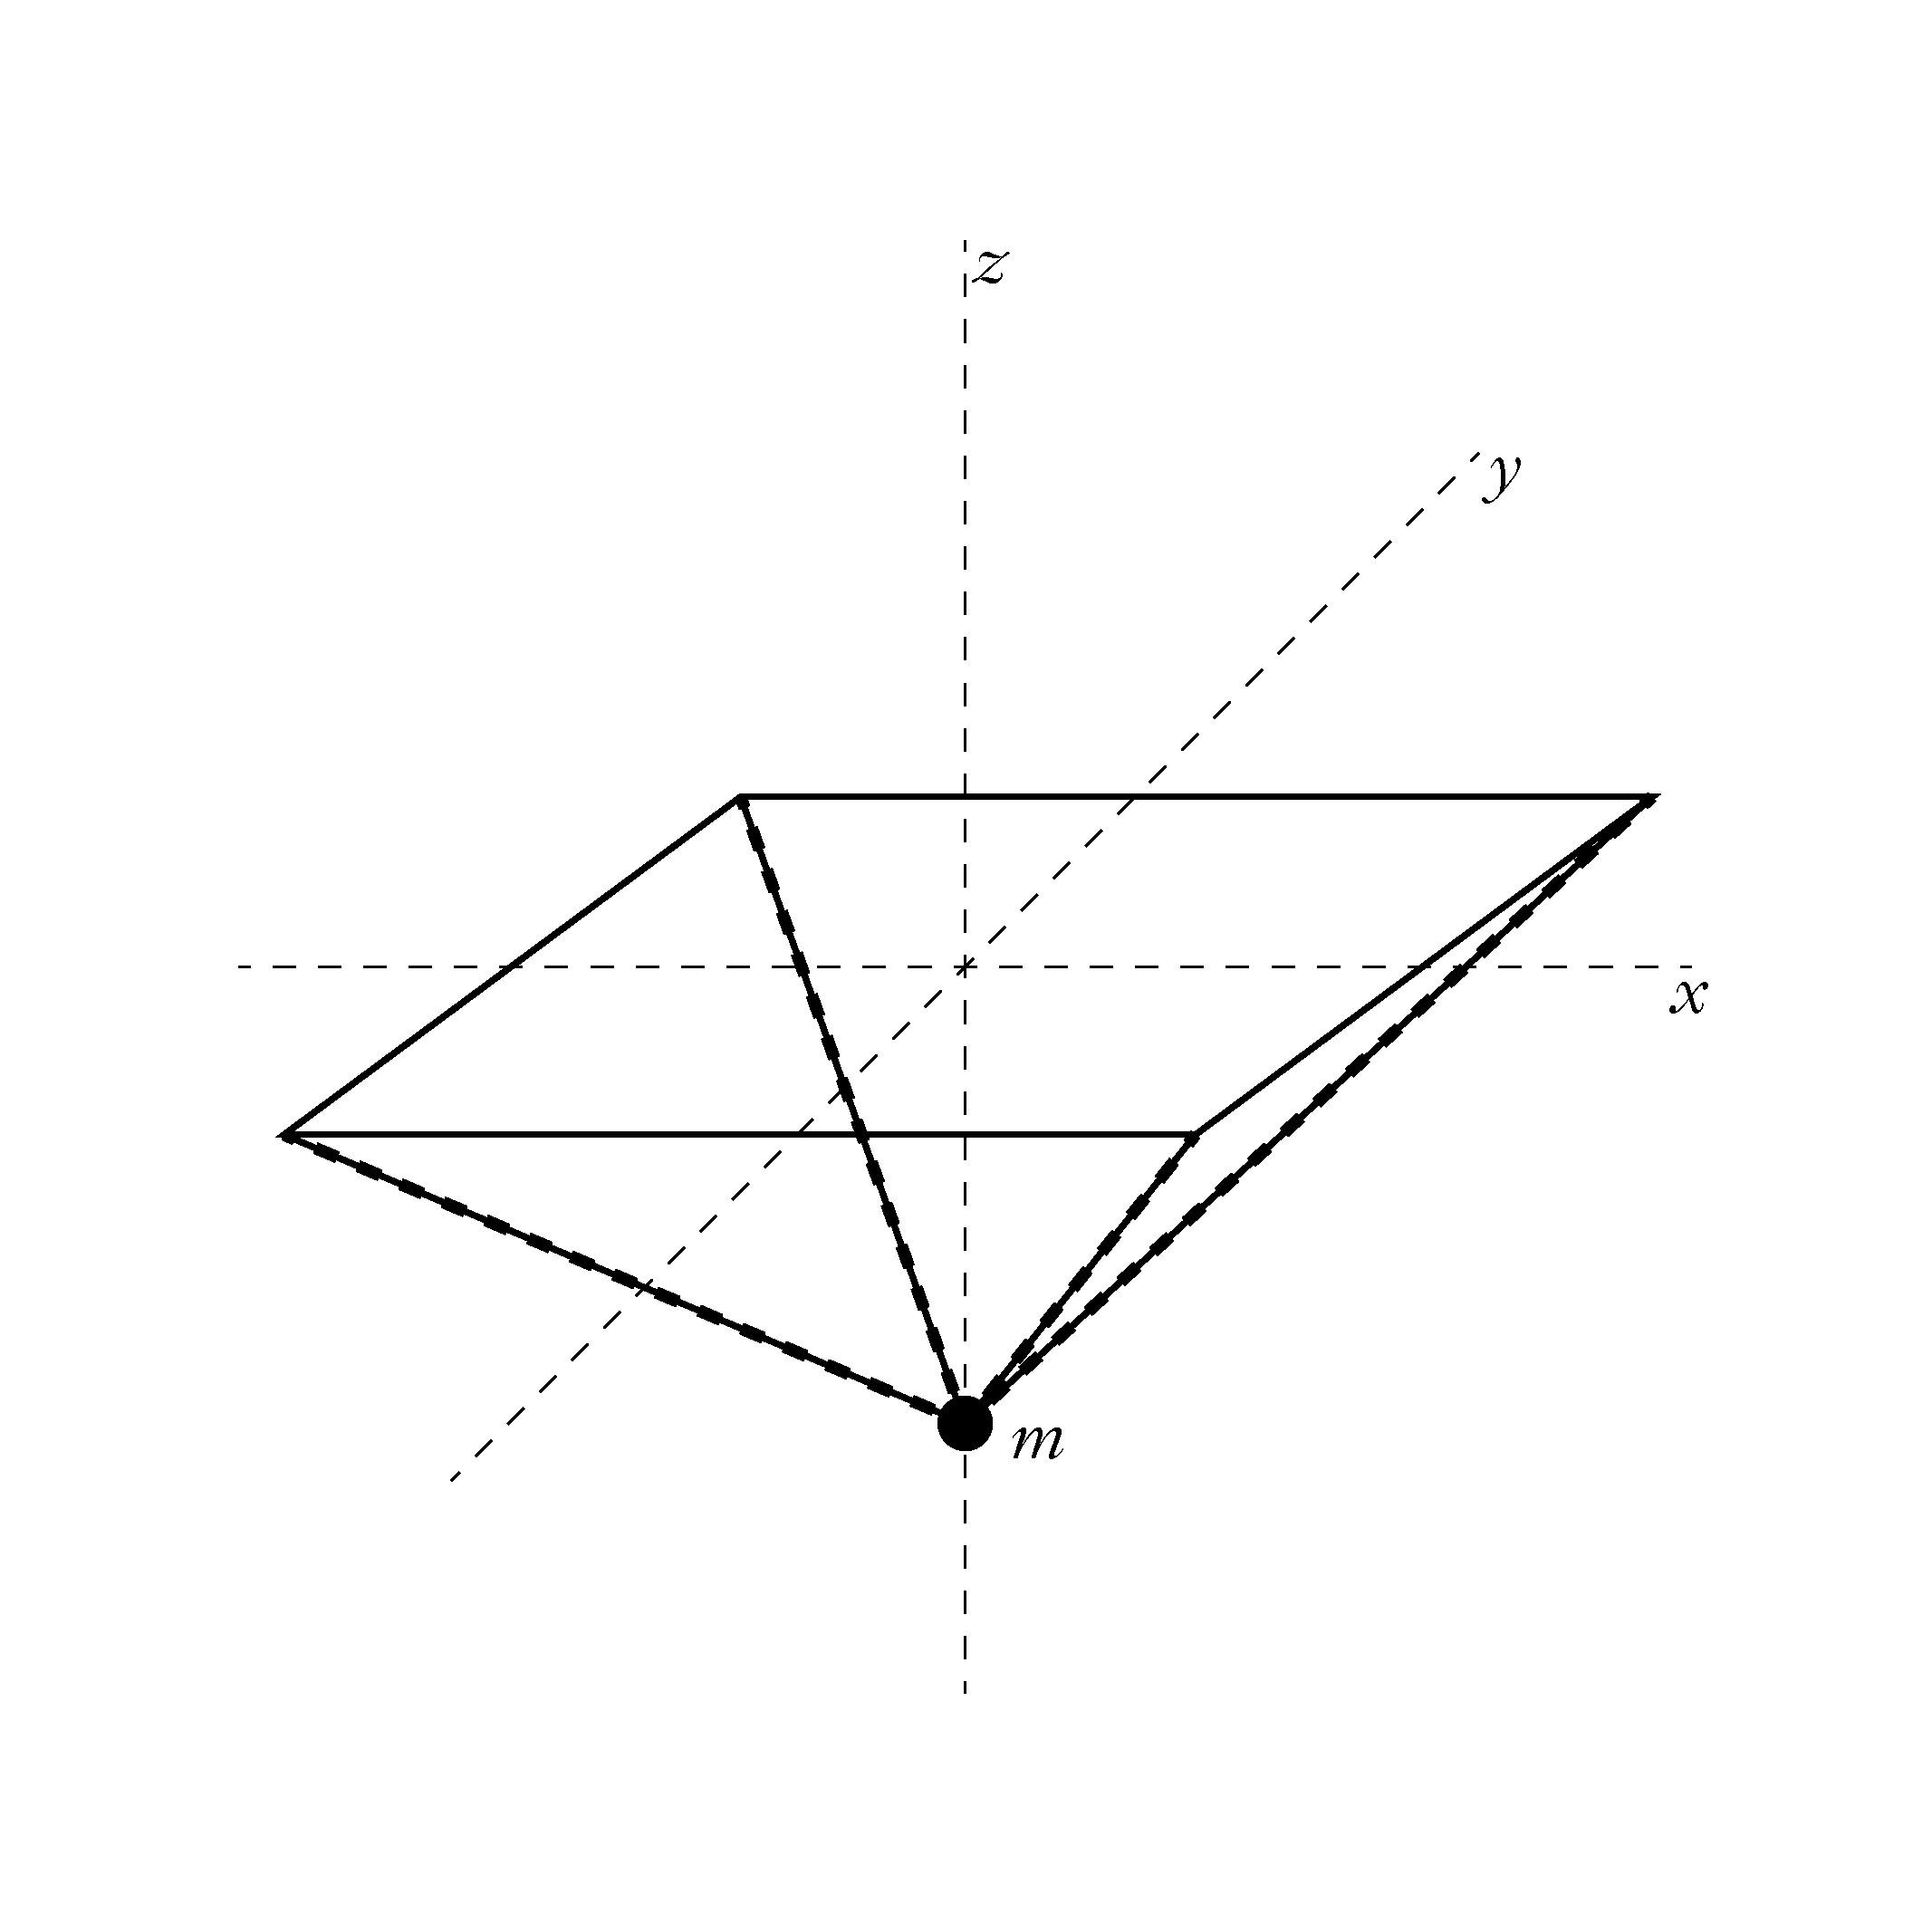
\includegraphics[height=4in]{plot.pdf}
        \end{center}


        First we can find taht the force on the mass for each spring is given as
        \begin{align*}
            \vv{F}_k &= -k\sqrt{(x\pm \frac{d}{2})^2 + (y\pm \frac{d}{2})^2 + z^2} \cdot \frac{(x\pm \frac{d}{2})\hat{x} + (y\pm \frac{d}{2}) \hat{y} + z\hat{z}}{\sqrt{(x\pm \frac{d}{2})^2 + y\pm \frac{d}{2})^2 + z^2}} \\
            & = -k(x\pm \frac{d}{2})\hat{x} + (y\pm \frac{d}{2}) \hat{y} + z\hat{z})
        \end{align*}
        Thus, we can easily to find the force on $x$ (or $y$) as
        \begin{align*}
            F_x &= \sum F_{kx} = -2k(x+ \frac{d}{2}) - 2k(x- \frac{d}{2}) \\
            &= -2k(2x) = -4kx
        \end{align*}
        Same we can find $F_y = -4kx$. And for $z$ we have:
        \begin{align*}
            F_z = F_g + \sum F_{kz} = -mg - 4 k z
        \end{align*}
        Now to find the potential, we can have:
        \[
        U_k = \frac{1}{2}(k_xx^2+k_yy^2+k_zz^2)
        \]
        where easy to see that $k_i = \ddot{U_i} = -\dot{F_i}$. Thus we have the vlaue of $k_i$ by differential force on each component, the reasult is just
        \[
        k_x = k_y = k_z = 4k
        \] 
        Therefore we have:
        \[
        U_k = 2(x^2+y^2+z^2)
        \]
        Moreover, we have $U_g = -mgz$ while we choose the origin in the equilibrium point. Thus, we can have the total potential energy as
        \[
        U = 2(x^2+y^2+z^2) - mgz
        \]
        To find the equilibrium point, we have:
        \begin{align*}
            F_z = -4kz - mg &= 0\\
            -4kz &= mg\\
            z &= - \frac{mg}{4k}
        \end{align*}
        Thus we have the equilibrium point at $(0,0,- \frac{mg}{4k})$.
        Thus we can have the total potential energy with respect to the center of the table as
        \[
        U = 2(x^2+y^2+z^2) + mg( \frac{mg}{4k} + z)
        \]
    \end{enumerate}
    \item Find the solution for the system in problem 1 with initial conditions:
    \[
    \vv{r}_i = \left(\frac{d}{2},0,0\right)\, , \, \dot{\vv{r}}_i = \left(0,A\frac{d}{2}\sqrt{\frac{k}{m}},0\right)
    \]\\

    From problem 1, we have for $x$ and $y$:
    \[
    F_x = m\ddot{x} = -4kx
    \]
    and for $z$ we have:
    \[
    F_z = m\ddot{z} = -4kz - mg
    \]

    Thus we have equations:
    \[
    \left\{
    \begin{aligned}
    m\ddot{x} &= -4kx \\
    m\ddot{y} &= -4ky \\
    m\ddot{z} &= -4kz - mg
    \end{aligned}
    \right. 
    \] 
    This is an easy differential equation, the solution is given as
    \[
    \left\{
    \begin{aligned}
    x &= \alpha_1 \sin(2\sqrt{\frac{k}{m}}t) + \alpha_2 \cos(2\sqrt{\frac{k}{m}}t)\\
    y &= \beta_1 \sin(2\sqrt{\frac{k}{m}}t) + \beta_2 \cos(2\sqrt{\frac{k}{m}}t)\\
    z &= \gamma_1 \sin(2\sqrt{\frac{k}{m}}t) + \gamma_2 \cos(2\sqrt{\frac{k}{m}}t) - \frac{gm}{4k}
    \end{aligned}
    \right. 
    \] 
    When $t = 0$, we have
    \[
    \left\{
    \begin{aligned}
    x &= \alpha_2\\
    y &= \beta_2\\
    z &= \gamma_2 - \frac{gm}{4k}
    \end{aligned}
    \right. 
    \] 
    with the initial value, we have
    \[
    \left\{
    \begin{aligned}
    \frac{d}{2} &= \alpha_2\\
    0 &= \beta_2\\
    \frac{gm}{4k} &= \gamma_2 
    \end{aligned}
    \right. 
    \] 
    Moreover, we have
    \[
    \left\{
    \begin{aligned}
    \dot{x} &= \alpha_1 2\sqrt{\frac{k}{m}}\cos(2\sqrt{\frac{k}{m}}t) - \alpha_2 2\sqrt{\frac{k}{m}}\sin(2\sqrt{\frac{k}{m}}t)\\
    \dot{y} &= \beta_1 2\sqrt{\frac{k}{m}}\cos(2\sqrt{\frac{k}{m}}t) - \beta_2 2\sqrt{\frac{k}{m}}\sin(2\sqrt{\frac{k}{m}}t)\\
    \dot{z} &= \gamma_1 2\sqrt{\frac{k}{m}}\cos(2\sqrt{\frac{k}{m}}t) - 2\sqrt{\frac{k}{m}}\gamma_2 \sin(2\sqrt{\frac{k}{m}}t)
    \end{aligned}
    \right. 
    \] 
    and when $t= 0$, we have
    \[
    \left\{
    \begin{aligned}
    0 &= \alpha_1 \\
    A\frac{d}{4} &= \beta_1\\
    0 &= \gamma_1
    \end{aligned}
    \right. 
    \]
    Easy to see 
    \[
    \left\{
    \begin{aligned}
    \alpha_1 &= 0\\
    \alpha_2 &= \frac{d}{2}\\
    \beta_1 &= A\frac{d}{4}\\
    \beta_2 &= 0\\
    \gamma_1 &= 0\\
    \gamma_2 &= \frac{gm}{4k}
    \end{aligned}
    \right. 
    \]
    Thus we have the answer as
    \[
    \left\{
    \begin{aligned}
    x &= \frac{d}{2} \cos(2\sqrt{\frac{k}{m}}t)\\
    y &= A\frac{d}{4} \sin(2\sqrt{\frac{k}{m}}t)\\
    z &= \frac{gm}{4k}\cos(2\sqrt{\frac{k}{m}}t) - \frac{gm}{4k}
    \end{aligned}
    \right. 
    \] 

    To make the motion a circle, we want the constants term is same for $x$ and $y$, i.e., $\frac{d}{2} = A\frac{d}{4}$. Thus, we have $A = 2$.

    \item Redo problem 1 for the case when the unstretched length of each spring is some finite positive value $l > 0$ \\

    Easy to see taht the energy is given as:
    \begin{align*}
        U_k =& \sum \frac{1}{2}k(\sqrt{(x\pm \frac{d}{2})^2 + y\pm \frac{d}{2})^2 + z^2}-l)^2 \\
          =& \frac{1}{2}k(\sqrt{(x + \frac{d}{2})^2 + (y + \frac{d}{2})^2 + z^2}-l)^2 \\
           &+\frac{1}{2}k(\sqrt{(x - \frac{d}{2})^2 + (y - \frac{d}{2})^2 + z^2}-l)^2 \\
           &+\frac{1}{2}k(\sqrt{(x + \frac{d}{2})^2 + (y - \frac{d}{2})^2 + z^2}-l)^2 \\
           &+\frac{1}{2}k(\sqrt{(x - \frac{d}{2})^2 + (y + \frac{d}{2})^2 + z^2}-l)^2 \\
        U =& U_k + U_g \\
          =& \frac{1}{2}k(\sqrt{(x + \frac{d}{2})^2 + (y + \frac{d}{2})^2 + z^2}-l)^2 \\
           &+\frac{1}{2}k(\sqrt{(x - \frac{d}{2})^2 + (y - \frac{d}{2})^2 + z^2}-l)^2 \\
           &+\frac{1}{2}k(\sqrt{(x + \frac{d}{2})^2 + (y - \frac{d}{2})^2 + z^2}-l)^2 \\
           &+\frac{1}{2}k(\sqrt{(x - \frac{d}{2})^2 + (y + \frac{d}{2})^2 + z^2}-l)^2 \\
           &-mgh(z)
    \end{align*}

    To find the force, for each spring we have:
    \begin{align*}
        \vv{F}_k &= -k(\sqrt{(x\pm \frac{d}{2})^2 + y\pm \frac{d}{2})^2 + z^2}-l) \cdot \frac{(x\pm \frac{d}{2})\hat{x} + (y\pm \frac{d}{2}) \hat{y} + z\hat{z}}{\sqrt{(x\pm \frac{d}{2})^2 + (y\pm \frac{d}{2})^2 + z^2}} \\
        & = -k(x\pm \frac{d}{2})\hat{x} + (y\pm \frac{d}{2}) \hat{y} + z\hat{z} +kl \cdot \frac{(x\pm \frac{d}{2})\hat{x} + (y\pm \frac{d}{2}) \hat{y} + z\hat{z}}{\sqrt{(x\pm \frac{d}{2})^2 + (y\pm \frac{d}{2})^2 + z^2}}
    \end{align*}
    Thus we have force on $x$ for each spring:
    \begin{align*}
        F_x &= -k(x\pm \frac{d}{2})+kl \cdot \frac{x\pm \frac{d}{2}}{\sqrt{(x\pm \frac{d}{2})^2 + (y\pm \frac{d}{2})^2 + z^2}} \\
        &= k(x\pm \frac{d}{2}) (\frac{l}{\sqrt{(x\pm \frac{d}{2})^2 + (y\pm \frac{d}{2})^2 + z^2}} -1)
        % &\approx k(x\pm \frac{d}{2}) (l(\frac{1}{(y\pm \frac{d}{2})^2 + z^2} - \frac{(x\pm \frac{d}{2})^2}{((y\pm \frac{d}{2})^2 + z^2)^2}) -1)
    \end{align*}
    and for $z$ for each spring we have
    \begin{align*}
        F_z &= -kz +kl \cdot \frac{z}{\sqrt{(x\pm \frac{d}{2})^2 + (y\pm \frac{d}{2})^2 + z^2}}\\
        &= kz (\frac{l}{\sqrt{(x\pm \frac{d}{2})^2 + (y\pm \frac{d}{2})^2 + z^2}}-1)
    \end{align*}

    To find the equilibrium point, we want all force are zero. Notice the equilbrium point sould in form of $0,0,z$ due to symmetry. Thus we now want to have $F_z = 0$
    \begin{align*}
        mg &= 4kz (\frac{l}{\sqrt{\frac{d^2}{2} + z^2}}-1) \\
        mg &= 4kz \frac{l}{\sqrt{\frac{d^2}{2} + z^2}}-4kz\\
        mg+4kz &= 4kz \frac{l}{\sqrt{\frac{d^2}{2} + z^2}} \\
        (mg+4kz)^2 &= 16k^2z^2 \frac{l^2}{\frac{d^2}{2} + z^2} \\
        m^2g^2+8kzmg+16k^2z^2 &=\frac{16k^2l^2z^2}{\frac{d^2}{2}+z^2} \\
        m^2g^2\frac{d^2}{2}+8kzmg\frac{d^2}{2}+16k^2z^2\frac{d^2}{2} 
        +m^2g^2z^2+8kz^3mg+16k^2z^4 &= 16k^2l^2z^2
    \end{align*}
        New we can just using the root formula to find $z$.

        To find $k_i$ for $x, y, z$, notice $\dot{F} = -\ddot{U} = k$. Thus we want to find the $\dot{F}$.
        For $x$, we have:
        \begin{align*}
            \frac{\de F}{\de x} = \frac{\de}{\de x}k(x\pm \frac{d}{2}) (\frac{l}{\sqrt{(x\pm \frac{d}{2})^2 + (y\pm \frac{d}{2})^2 + z^2}} -1)
        \end{align*}
        Around the equilibrium point, we can just let $y = 0$, and by set the origin point at equilibrium point, $z = 0$.
        \begin{align*}
            \frac{\de F}{\de x} &= \frac{\de}{\de x}k(x\pm \frac{d}{2}) (\frac{l}{\sqrt{(x\pm \frac{d}{2})^2 + \frac{d^2}{4}}} -1)\\
            &= \frac{d^2l k}{\sqrt{2}(d^2+2dx+2x^2)^\frac{3}{2}}
        \end{align*}
        around equilibrium point, $x = 0$, thus we have
        \[
        k_x = \frac{l k}{\sqrt{2}d}
        \]
        and $y$ are the same.

        For $z$, we have
        \begin{align*}
            \frac{\de F}{\de z} &= kz (\frac{l}{\sqrt{\frac{d^2}{2} + z^2}}-1)\\
            &= \frac{\sqrt{2}d^2l}{(d^2+2z^2)^\frac{3}{2}} - 1\\
            &= \frac{\sqrt{2}l}{d} - 1
        \end{align*}


        Thus we have:
        \[
        U_i \approx U_i(0) + \dot{U}_i(0)i + \frac{1}{2}\ddot{U}(0)i^2 = \frac{1}{2}\ddot{U}(0)i^2
        \]
        that is:
        \[
        U = \frac{1}{2} (k_xx^2+k_yy^2+k_zz^2)
        \]
        where $k_x = k_y = \frac{l k}{\sqrt{2}d}$, $k_z = \frac{\sqrt{2}l}{d} - 1$


    % To find the equilibrium point, we want to have point where $\dot{U} = 0$. Easy to see that the the equilibrium is in form $(0,0,z)$ due to symmetry. Thus we have:
    % \begin{align}
    %     \frac{\partial U}{\partial z} =& \frac{\de U}{\de z} \\
    %       =& \frac{\de U}{\de z}2k(\sqrt{\frac{d^2}{2} + z^2}-l)^2-mgh(z) \\
    %       =& \frac{4kz(\sqrt{\frac{d^2}{2}+z^2}-l)}{\sqrt{\frac{d^2}{2}+z^2}} - mg = 0 \\
    %       =& 4kz - \frac{4kzl}{\sqrt{\frac{d^2}{2}+z^2}} -mg = 0
    % \end{align}
    % Thus we have
    % \begin{align*}
    %     4kz - \frac{4kzl}{\sqrt{\frac{d^2}{2}+z^2}} &= mg \\
    %     \frac{16k^2z^2l^2}{\frac{d^2}{2}+z^2} &= (mg - 4kz)^2 \\
    %     \frac{16k^2z^2l^2}{\frac{d^2}{2}+z^2} &= m^2g^2 - 8kzmg +16k^2z^2 \\
    %     16k^2l^2 &= (m^2g^2 - 8kzmg +16k^2z^2)(\frac{d^2}{2z^2}+1)\\
    %     16k^2z^2l^2 &= m^2g^2\frac{d^2}{2} - 8kzmg\frac{d^2}{2} +16k^2z^2\frac{d^2}{2} + m^2g^2z^2 - 8kz^3mg +16k^2z^4 \\
    %     m^2g^2\frac{d^2}{2} &=(16k^2l^2 -16k^2\frac{d^2}{2}  - m^2g^2)z^2 + 8kzmg\frac{d^2}{2} + 8kz^3mg -16k^2z^4 \\
    % \end{align*}
    % Thus by plug it into the root formula to find $z$ of equilibrium point.




    % \begin{align*}
    %         \vv{F}_k &= -k(\sqrt{(x\pm \frac{d}{2})^2 + y\pm \frac{d}{2})^2 + z^2}-l) \cdot \frac{(x\pm \frac{d}{2})\hat{x} + (y\pm \frac{d}{2}) \hat{y} + z\hat{z}}{\sqrt{(x\pm \frac{d}{2})^2 + (y\pm \frac{d}{2})^2 + z^2}} \\
    %         & = -k(x\pm \frac{d}{2})\hat{x} + (y\pm \frac{d}{2}) \hat{y} + z\hat{z} +kl \cdot \frac{(x\pm \frac{d}{2})\hat{x} + (y\pm \frac{d}{2}) \hat{y} + z\hat{z}}{\sqrt{(x\pm \frac{d}{2})^2 + (y\pm \frac{d}{2})^2 + z^2}}
    % \end{align*}
    % Thus we have for $x$ (and $y$)
    % \begin{align*}
    %     F_x &= -k(x\pm \frac{d}{2})+kl \cdot \frac{x\pm \frac{d}{2}}{\sqrt{(x\pm \frac{d}{2})^2 + (y\pm \frac{d}{2})^2 + z^2}} \\
    %     &= k(x\pm \frac{d}{2}) (\frac{l}{\sqrt{(x\pm \frac{d}{2})^2 + (y\pm \frac{d}{2})^2 + z^2}} -1)
    %     % &\approx k(x\pm \frac{d}{2}) (l(\frac{1}{(y\pm \frac{d}{2})^2 + z^2} - \frac{(x\pm \frac{d}{2})^2}{((y\pm \frac{d}{2})^2 + z^2)^2}) -1)
    % \end{align*}
    % and for $z$ we have
    % \begin{align*}
    %     F_z &= -kz +kl \cdot \frac{z}{\sqrt{(x\pm \frac{d}{2})^2 + (y\pm \frac{d}{2})^2 + z^2}}\\
    %     &= kz (\frac{l}{\sqrt{(x\pm \frac{d}{2})^2 + (y\pm \frac{d}{2})^2 + z^2}}-1)
    % \end{align*}
    %%%%

    \item Fouries Series
    \begin{enumerate}
        \item Find the fourier series corresponding to a square wave with amplitude $\frac{F}{m}$ and period $T$\\

        Given
        \begin{align*}
            s(x) &= +1 \, \text{for} \, x \in (0,\frac{T}{2})\\
                 &= -1 \, \text{for} \, x \in (\frac{T}{2},0)
        \end{align*}
        and we have
        \begin{align*}
            a_n &= \frac{2}{T}\int_0^T s(x)\cos(\frac{2\pi n x}{T})\de x \\
                &= \frac{2}{T}(\int_0^{\frac{T}{2}} \cos(\frac{2\pi n x}{T})\de x  - \int_\frac{T}{2}^T \cos(\frac{2\pi n x}{T})\de x ) \\
                &= 0
        \end{align*}
        and same for $b_n$
        \begin{align*}
            b_n &= \frac{2}{T}\int_0^T s(x)\sin(\frac{2\pi n x}{T})\de x \\
                &= \frac{2}{T}(\int_0^{\frac{T}{2}} \sin(\frac{2\pi n x}{T})\de x  - \int_\frac{T}{2}^T \sin(\frac{2\pi n x}{T})\de x ) \\
                &= -\frac{2}{T} (\frac{T}{2\pi n}\cos(\frac{2\pi n x}{T})]_0^{\frac{T}{2}} - \frac{T}{2\pi n}\cos(\frac{2\pi n x}{T})]_\frac{T}{2}^T)\\
                &= -\frac{2}{T} \frac{T}{2\pi n}(\cos(\pi n) - \cos(0) - \cos(2\pi n) + \cos(\pi n)\\
                &= -\frac{1}{\pi n}(-1 + \cos(\pi n))\\
                &= \frac{1}{\pi n}(1-\cos(\pi n x))
        \end{align*}
        Thus we have
        \[
            s(x) = \frac{F}{m}\sum_0^\infty b_n \sin(\frac{2\pi n x}{T})
        \]
        while $b_n$ is given as above.

        \item Find the steady state solution for a one-demensional damped harmonic oscillator subject to this driving force.\\

        From the above we can see that the driving force is given as the sum of all cos wave. Thus we can say that solution of the oscillator is just a linear combination of the solution of each cos wave, i.e.,
        \[
        x(t) = \sum_0^\infty A_n \sin(n\omega t - \varphi_n)
        \]
        where
        \begin{align*}
            A_n &= \frac{b_n}{m} \frac{1}{\sqrt{(\omega_0^2 - n^2\omega^2)^2 + 4\beta^2n^2\omega^2}} \\
            \varphi_n &= \tan^{-1}(\frac{2\beta n\omega}{\omega_0^2-n^2\omega^2}) 
        \end{align*}
    \end{enumerate}
    \item A rubber band that is stretched more than a tiny bit is not a very good approximation to a harmonic oscillator. Suppose its potential is
    \[
    U(x) = \frac{1}{2}k(x-l)^2 + \frac{1}{3}a(x-l)^3 + \frac{1}{4}b(x-l)^4
    \]
    where $a, b$ are small positive.
    \begin{enumerate}
        \item Sketch the potential for $k = 1$, $a = \frac{1}{2}$, $b = \frac{1}{8}$
        \item Show taht the only stable equilibrium point is still at $x = l$\\

        Let shift the coordinate system $l$ so that now $x = (x'-l)$ for $x'$ in the old system. Thus we have:
        \[
            U(x) = \frac{1}{2}kx^2 + \frac{1}{3}ax^3 + \frac{1}{4}bx^4
        \]
        easy to find
        \[
        \dot{U} = kx + ax^2 + bx^3
        \]
        and
        \[
        \ddot{U} = k + 2ax + 3bx^2
        \]
        we can see that when $x = 0$ ($x' = l$), we have a an $U_\text{min}$, i.e., it is a stable equilbrium point.

        Moreover, we have two more point where $\dot{U} = 0$:
        \[
        x = \pm\frac{\sqrt{a^2-4bk}-a}{2b}
        \]
        when we plug it into $\ddot{U}$, easy to see $\ddot{U}<0$, which give us a unstable equilbrium point.
        \item Find the frequency of small oscillations about this point.\\

        Easy to see that at the equilibrium point, $U(0) = \dot{U} = 0$. Thus we have:
        \[
        U(x) \approx U(0) + \dot{U}(0)x + \frac{1}{2}\ddot{U}(0)x^2 = \frac{1}{2}kx^2
        \]
        Thus we have $\omega_0^2 = \frac{k}{m}$.

    \end{enumerate}
\end{enumerate}


% \begin{eqnarray*}
\end{document}